\documentclass{article}
\usepackage{graphicx} % Required for inserting images
\usepackage[english]{babel}
\usepackage{amsmath}
\usepackage{amsfonts}
\usepackage{amsthm}
\usepackage{amssymb}
\usepackage{physics}

\usepackage{mathtools}


\numberwithin{equation}{section}

\newcommand{\Set}[1]{\{#1\}}
\newcommand{\FT}{\mathcal{F}}
\newcommand\perm[2][^n]{\prescript{#1\mkern-2.5mu}{}P_{#2}}
\newcommand\comb[2][^n]{\prescript{#1\mkern-0.5mu}{}C_{#2}}

\DeclareMathOperator{\spn}{span}

\makeatletter
\renewcommand*\env@matrix[1][*\c@MaxMatrixCols c]{%
  \hskip -\arraycolsep
  \let\@ifnextchar\new@ifnextchar
  \array{#1}}
\makeatother

\newtheorem{theorem}{Theorem}[section]
\newtheorem{corollary}{Corollary}[theorem]
\newtheorem{lemma}[theorem]{Lemma}
\title{Problem Presentation 5}
\author{Siyu Chen}
\date{July 2023}

\begin{document}

\maketitle

\section{Introduction of Section 3, page 632: problem 4}

At t = 0, two flat slabs each 5 cm thick, one at $0^\circ$ and one at $20^\circ$, are stacked together, and then the surfaces are kept at $0^\circ$. Find the temperature as a function of $x$ and $t$ for $t > 0$.

This is a Partial Differential Equations of Heat Diffusion, described by:

\begin{align}
    \frac{\partial^2 u}{\partial x^2} = \frac{1}{\alpha^2} \frac{\partial u}{\partial t}
\end{align}

We must find the solution that makes sense with our boundary conditions given, and graph it on a computer. This is a common PDE that appears in physics. The solution to this boundary condition problem must make physical sense of how the heat is flowing. We can intuitively predict that, since there is no external heat source and the surrounding environment has a temperature of $0^\circ$, that our slab will cool down over time. Computer graph will help us better visualize that. We can use separation of variables to approach this problem.

\section{Relation to course material}

We have been discussing simple PDEs in physics and using Separations of Variables to solve it. We must find the general solution of this partial differential equation, and apply our boundary conditions to restrict our constants in the solution. Finally, we would have to use Fourier Series to expand our function to match the initial condition of the slab. This is something that we have been covering as well in the course.

\section{Steps to solve the problem }

Our initial conditions for our $u(x,t)$ are:

\begin{align}
    u(0, t) &= u(20, t) = 0^\circ \\
    u(x, 0) &= 20^\circ \quad 0 < 5 < 10
\end{align}

Since our system only concerns the $x$-direction, we can use the diffusion heat equation:

\begin{align}
    \frac{\partial^2 u}{\partial x} = \frac{1}{\alpha^2} \frac{\partial u}{\partial t}
\end{align}

now using separation of variables:

\begin{align}
    u(x,t) = X(x)T(t)
\end{align}

and our equation becomes:

\begin{align}
    T(t) \frac{\partial^2 X}{\partial x^2} = \frac{1}{\alpha^2} X(x) \frac{\partial T}{\partial t} 
\end{align}

rearranging and equating each side to constant, we have:

\begin{align}
    \frac{1}{X(x)} \frac{\partial^2 u}{\partial x^2} = \frac{1}{\alpha^2} \frac{1}{T(t)} \frac{\partial T}{\partial t} = -k^2
\end{align}

solving for each differential equations, we can obtain the following: 

\begin{align}
    T(t) = t_0 e^{-k^2 \alpha^2 t} \quad X(x) = x_1 \cos(kx) + x_2 \sin(kx)
\end{align}

Now, to satisfy our boundary condition, we can see that since at $x = 0, u = 0$ from our boundary condition, we can discard our $\cos(kx)$ term as $\cos(0) = 1$. We then can write our solution in the form of:

\begin{align}
    u(x,t) = A \sin(kx) e^{-k^2 \alpha^2 t}
\end{align}

where $A$ is a constant. Now to satisfy our initial conditions, we have:

\begin{align}
    u(x,0) = A \sin(kx) = \begin{cases}
        20^\circ \quad &(0<x<5) \\
        0^\circ \quad &(5<x<10)
    \end{cases} 
\end{align}

This is a Fourier Series problem and from our boundary condition, our solution must be in the form of:

\begin{align}
    u(x,0) = \sum_{n=0}^{\infty} b_n \sin \frac{n \pi x}{10} 
\end{align}

Evaluating for our constants, we have:

\begin{align}
    b_n = \frac{1}{10}\int_{0}^{10} f(x) \sin \frac{n \pi x}{10} = 2 \int_{5}^{10} \sin \frac{n\pi x}{10} = \frac{40}{\pi n} ( \cos(\frac{\pi n}{2}) - \cos(\pi n))
\end{align}

we can then write our solution in terms of a series as:

\begin{align}
    u(x,t) = \frac{40}{\pi} \sum_{n=1}^{\infty} \frac{1}{n} ( \cos(\frac{\pi n}{2}) - \cos(\pi n)) \sin \frac{n\pi x}{10} e^{-\alpha^2 \frac{n^2\pi^2}{100}t}
\end{align}

Wolfram Alpha gives the following graphs, this is a $x-t$ graph. Since the slab temperature has no $y,z$ dependencies, this is the cross-section of $x$ extended in time. The value chosen is $n=100, \alpha = 1$

\begin{figure}[!htb]
   \begin{minipage}{0.48\textwidth}
     \centering
     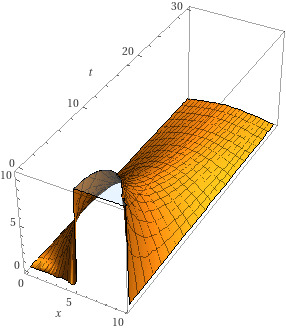
\includegraphics[width=.7\linewidth]{plot3.1.jpg}
     \caption{3-D map of $u(x,t)$}\label{Fig: 3.1}
   \end{minipage}\hfill
   \begin{minipage}{0.48\textwidth}
     \centering
     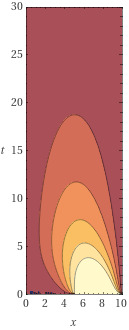
\includegraphics[width=.7\linewidth]{plot3.2.jpg}
     \caption{Contour map of $u(x,t)$}\label{Fig: 3.2}
   \end{minipage}
\end{figure}

We can see that this graph makes sense as, without additional heat source, the high temperature slab begins to gradually lose its temperature over time to the environment kept at $0^\circ$ while conducting some heat to the adjacent slab.

\section{Solution Summary}

We use separation of variables to solve for the general solution of the heat diffusion equation, and then apply our boundary conditions to restrict our solutions to describe the physical system. Finally, we graph the solution to see that it does, indeed, make sense as heat diffuses away as time goes on.

\section{Note on method}

We use basic methods to solve 2nd order and 1st order homogeneous ODEs when we do separations of variables. After that, we use Fourier Series to describe the initial condition that the region $x \in [5, 10]$ is at a higher temperature than the rest. We compute back the time dependent portion of our solution, and obtain our result.


\end{document}
